\chapter{Problem definition and background}\label{chapt:problem}
Road digitalization is an expensive operation. Research is being done to identify roads automatically using Artificial Intelligence with the different types of images. High-resolution satellite images are expensive to get, and covering an entire state or country is a nightmare. Mid-resolution satellite images, on the other hand, can be obtained for free, but identification of roads on mid-resolution(>5~m) satellite data is difficult and often has low accuracy. This work tries to detect the smaller roads(with 1 or 2 lanes) which are often missed out. \par

We will be using RGB images from satellite sentinel-2A. Detailed parameters of the satellite are given in Table~\ref{tab:sentinel-resolution}. Band 2(Blue), 3(Green), and 4(Red) are stacked together to get the a 3-channel RGB image. As seen in the specifications, the spacial resolution of the final image is 10m. The task is to increase the accuracy of the existing road-detection algorithm. \par

\begin{table}[h!]
  \centering
  \begin{tabular}{ |c|c|c| }
    \hline
    Spatial Resolution(m) & Band Number & Central Wavelength (nm) \\
    \hline
    10&2&492.4 \\
    10&3&559.8 \\
    10&4&664.6 \\
    10&8&832.8 \\
    20&5&704.1 \\
    20&6&740.5 \\
    20&7&782.8 \\
    20&8a&864.7 \\
    20&11&1613.7 \\
    20&12&2202.4 \\
    60&1&442.7 \\
    60&9&945.1 \\
    60&10&1373.5 \\
    \hline\\
  \end{tabular}
  \caption{Wavelengths and Bandwidths of the three Spatial Resolutions of the MSI instruments \cite{sentinelSpecifications}}
  \label{tab:sentinel-resolution}
\end{table}

On combining the three bands from raw satellite image, the resulting image size is of the order of 400~MB for 1 mid-sized city. At first, this may not seem large on comparison with some of the media files. But handling files of this size in DCNN is a serious issue. Let's see the specifications needed by a computer to handle this image in 1 go:
% TODO: Calculations showing 400MB in DCNN

\par
This might be possible for massive supercomputers, but a general workstation has RAM anywhere from 128 to 256 GB RAM, while personal computers range from 8 GB to 32 GBs RAM. Thus, this image must be divided into several parts so that out algorithms work on a easily available device. \par

Our input image doesn't have sifficiently high resolution to identify small roads. To deal with this problem of pixelization, we will be using two types of models. This setup is shown in Figure~\ref{fig:model_complete_without_labels}. Unless specifically mentioned, a model means a combined setup using super-resolution and road-detection models. Data from input layer goes to the super-resolution model which is consequently passed to the road-detection model. The final output consists of the predicted road network in image. \par

\begin{figure}
  \centering
  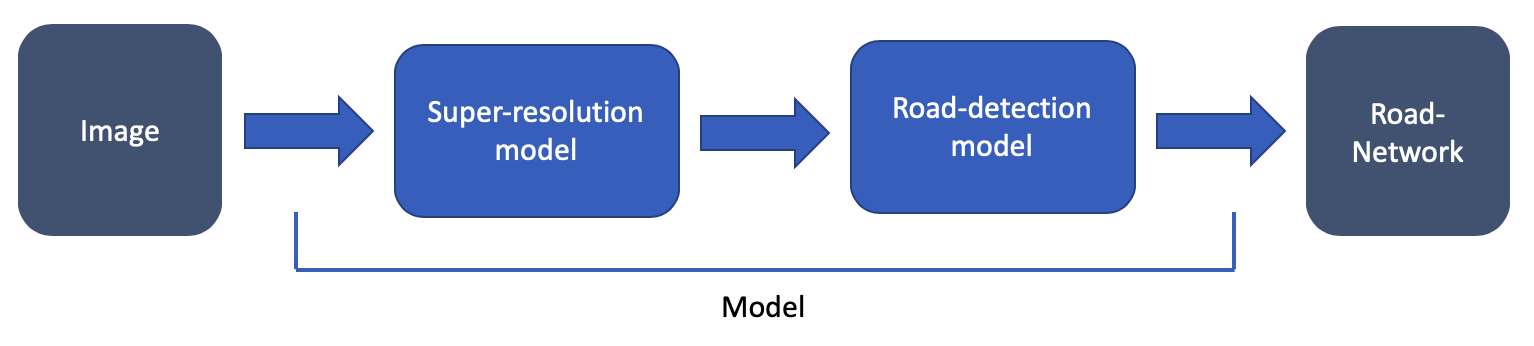
\includegraphics[width=\textwidth]{model_complete_without_labels}
  \caption{Complete setup: Combination of Super-resolution and road-detection models.}
  \label{fig:model_complete_without_labels}
\end{figure}
